\newcommand{\thiefDescription}{
\section{Thief}
    \epigraph{\textit{"Marek, always helpful, said that the UnderTyr
    catacombs are supposed to be haunted. Think I'll go make
    some inquiries about where a 'heretic' like me can get some
    holy earth. Always go prepared...."}}{ Janos, human rogue }

    The thief pilfers what she can, knows her way around the labyrinth of the warrens of the city and knows the best fences and suppliers of illegal goods.
    Skullduggery and Stealth are her livelihood, while Streetwise and her knowledge of the Underworld ensures she knows her way around town.\\
    \\
    See \nref{tlttree:thief} for more information.
}

\newcommand{\thiefTree}{
    \newpage
    \subsection{Thief Talent Tree}
    \label{tlttree:thief}

    \textbf{Class Skills:} Skullduggery, Stealth, Streetwise, Knowledge (Underworld)
    \newline

    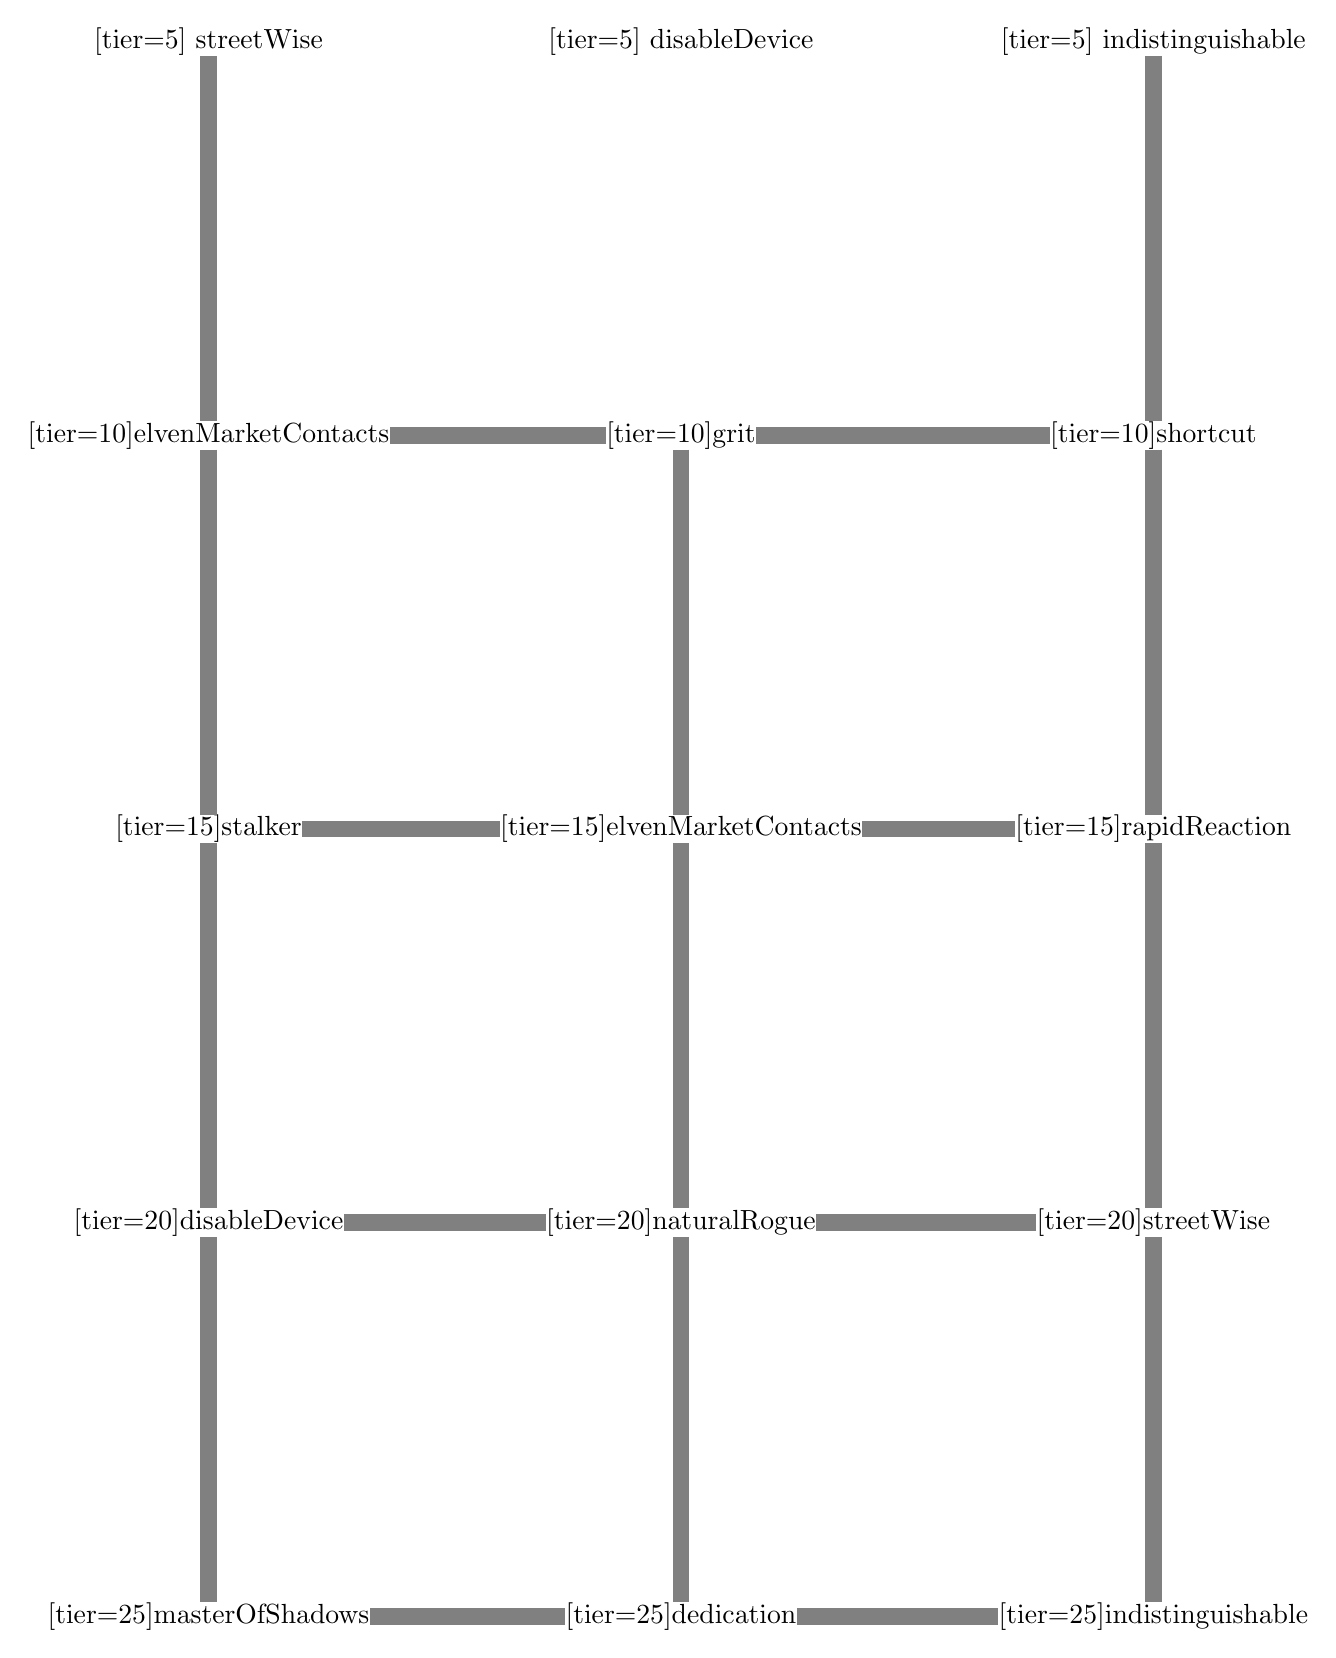
\begin{tikzpicture}
        \draw ( 0,  0) node(aa)[inner sep=0]{\TalentBox[tier=5] {streetWise}}
              ( 6,  0) node(ab)[inner sep=0]{\TalentBox[tier=5] {disableDevice}}
              (12,  0) node(ac)[inner sep=0]{\TalentBox[tier=5] {indistinguishable}}
              ( 0, -5) node(ba)[inner sep=0]{\TalentBox[tier=10]{elvenMarketContacts}}
              ( 6, -5) node(bb)[inner sep=0]{\TalentBox[tier=10]{grit}}
              (12, -5) node(bc)[inner sep=0]{\TalentBox[tier=10]{shortcut}}
              ( 0,-10) node(ca)[inner sep=0]{\TalentBox[tier=15]{stalker}}
              ( 6,-10) node(cb)[inner sep=0]{\TalentBox[tier=15]{elvenMarketContacts}}
              (12,-10) node(cc)[inner sep=0]{\TalentBox[tier=15]{rapidReaction}}
              ( 0,-15) node(da)[inner sep=0]{\TalentBox[tier=20]{disableDevice}}
              ( 6,-15) node(db)[inner sep=0]{\TalentBox[tier=20]{naturalRogue}}
              (12,-15) node(dc)[inner sep=0]{\TalentBox[tier=20]{streetWise}}
              ( 0,-20) node(ea)[inner sep=0]{\TalentBox[tier=25]{masterOfShadows}}
              ( 6,-20) node(eb)[inner sep=0]{\TalentBox[tier=25]{dedication}}
              (12,-20) node(ec)[inner sep=0]{\TalentBox[tier=25]{indistinguishable}}
        ;

        \tikzstyle{bar}=[gray,-,>=stealth, line width=6pt]

        \draw [bar] (aa) to (ba);
        \draw [bar] (ac) to (bc);
        \draw [bar] (ba) to (ca);
        \draw [bar] (bb) to (cb);
        \draw [bar] (bc) to (cc);
        \draw [bar] (ca) to (da);
        \draw [bar] (cb) to (db);
        \draw [bar] (cc) to (dc);
        \draw [bar] (da) to (ea);
        \draw [bar] (db) to (eb);
        \draw [bar] (dc) to (ec);

        \draw [bar] (ba) to (bb);
        \draw [bar] (bc) to (bb);

        \draw [bar] (ca) to (cb);
        \draw [bar] (cc) to (cb);

        \draw [bar] (da) to (db);
        \draw [bar] (dc) to (db);

        \draw [bar] (ea) to (eb);
        \draw [bar] (ec) to (eb);
    \end{tikzpicture}
}
